%%%%%%%%%%%%%%%%%%%%%%%%%
%% Chapter 2: Showcase %%
%%%%%%%%%%%%%%%%%%%%%%%%%

\chapter{Showcase}
\label{chap:showcase}
\Cref{sec:acr_refs} shows examples of the usage of the package \texttt{glossaries} and of adding citations. \Cref{sec:subsection} displays what subsections look like in this template, and \cref{sec:math} showcases a large variety of math symbols and equations. The last section, \cref{sec:text}, shows a large patch of text with some (wrap)figures and table.

\section{Acronyms and references}
\label{sec:acr_refs}
Here is a nice acronym test: two big \glspl{gc} are \gls{pal5} and \gls{m5}. \Gls{m6} is an open cluster, whereas \gls{m31} is a galaxy. Here is another acronym that starts with a "p": \gls{pca}. When acronyms are referenced a second time, it only shows the short name: \gls{pal5}, \gls{m5}. One single \gls{gc}, and multiple \glspl{gc}. One \gls{agn}, multiple \glspl{agn}, and multiple long \glsxtrlongpl{agn}. This is an example of an unclickable short reference, \glsfmtshort{vlt}, an unclickable long reference, \glsfmtlong{vlbi}, and an unclickable plural form of a short reference \glsfmtshortpl{gc}. Unclickable references do not show up in the nomenclature if they are not referred to anywhere else in the text. You will see that \gls{vlbi} is listed in the nomenclature, but \glsfmtshort{vlt} is not. 

This is an example of a paragraph with in-text
citations using the aasjournal BibTeX style.
Here is a reference to a journal article with
a single author \citep{article}, to a journal
article with two authors without parenthesis \citet{article2}, and to a journal article with six authors \citep{article6}. Here is a citation to a book \citep{book}.

\section{Subsectionceptionsection}
\label{sec:subsection}
This is the first section of the subsectionceptionsection. Let's start with some text. \lipsum[66]
\subsection{Subsection of the first section}
Look, its a subsection.
\subsection{Another subsection}
And there is more!
\subsection{Third's a charm}
Welcome to the final subsection.

\section{Math}
\label{sec:math}
\def\ii{\mathrm{i}}
\def\pp{\mathrm{\pi}}

Basic examples of equations:
\begin{itemize}
\item Moment of inertia:
\begin{align}
    \sum_{i=1}^N m_i\vec{r_i}^2
\end{align}
  \item Einstein's field equations:
    \begin{align}
        G_{\alpha\beta} &\equiv R_{\alpha\beta}-\frac{1}{2} g_{\alpha\beta}R+\Lambda g_{\alpha\beta}=\frac{8\pi\kappa}{c^2}T_{\alpha\beta}
    \end{align}
\item Main-sequence relations:
    \begin{align} 
    \qquad \frac{L}{\si\lsun} &= 
    \left\{
    \begin{aligned}
     &0.35\left(\frac{M}{\si\msun}\right)^{2.62}, &M&<0.7\si\msun \\
     &1.02\left(\frac{M}{\si\msun}\right)^{3.92}, &M&\geq 0.7\si\msun
    \end{aligned}
    \right.                                                 \label{eq:mass_light} \\
        \qquad \frac{R}{\si\rsun} &= 
    \left\{
    \begin{aligned}
     &1.06\left(\frac{M}{\si\msun}\right)^{0.945}, &M&<1.66\si\msun \\
     &1.33\left(\frac{M}{\si\msun}\right)^{0.555}, &M&\geq 1.66\si\msun
    \end{aligned}
    \right.                                                 \label{eq:radius_mass} 
    \end{align} 
\item Wave functions:
\begin{align}
\Phi(k,t)&=\frac{1}{\sqrt{h}}\int\Psi(x,t){\rm e}^{-ikx}dx,  
&\Psi(x,t)&=\frac{1}{\sqrt{h}}\int\Phi(k,t){\rm e}^{ikx}dk \\
\langle f(t)\rangle &=\iiint\Psi^* f\Psi d^3V, &\langle f_p(t)\rangle &=\iiint\Phi^*f\Phi d^3V_p
\end{align}
\item Wave equation:
\begin{align}
\nabla^2u-\frac{1}{v^2}\QQ{u}{t}=\QQ{u}{x}+\QQ{u}{y}+\QQ{u}{z}-\frac{1}{v^2}\QQ{u}{t}=0
\end{align}


\end{itemize}

\section{Text and figures}
\label{sec:text}
\begin{wrapfigure}{r}{0.5\textwidth}
    \vspace{-1em}   % sometimes needed to align the image, 1 em is size of capital M, 1 ex of lower case x
	\centering
	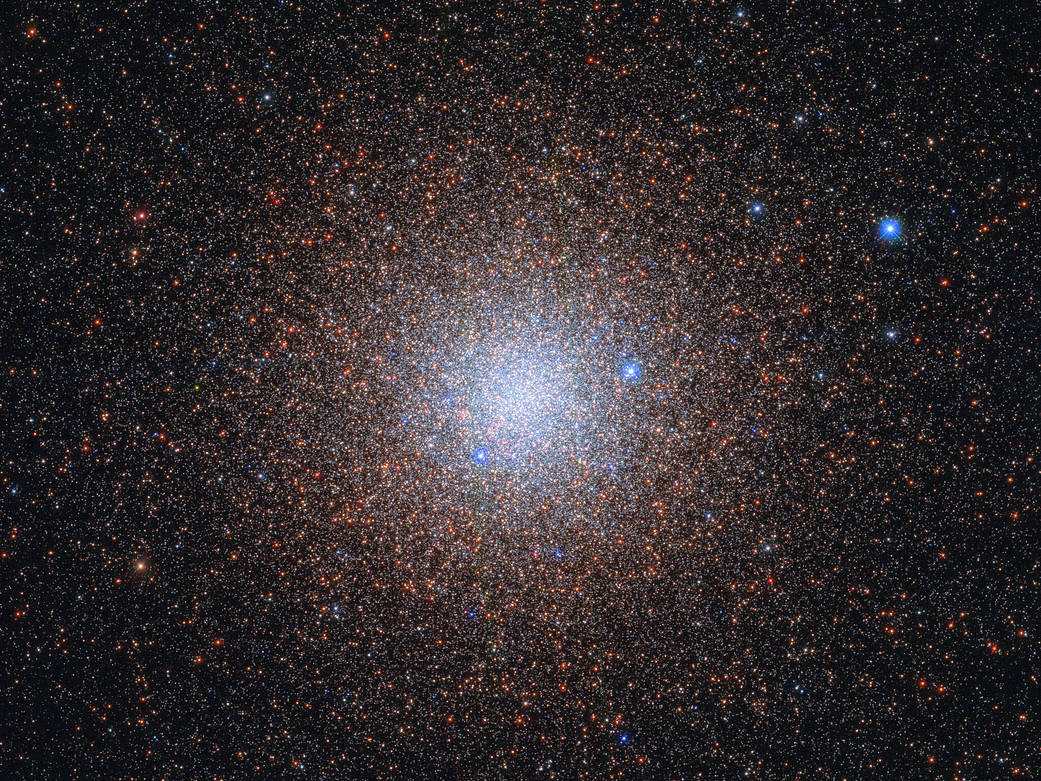
\includegraphics[width=0.5\textwidth]{figures/gc_image.jpg}
	\caption[A picture of NGC 6441.]{A picture of NGC 6441, one of the most massive and luminous GCs in the Milky Way.}
	\label{fig:prettypicture}
	\imref{Image credit: ESA/Hubble \& NASA, G. Piotto}
    %\vspace{-1ex}
\end{wrapfigure}
Check out \cref{fig:prettypicture}, \cref{fig:NGC1300} and \cref{tab:example_table}!
\lipsum[1-3]

\begin{table}[t]
    \centering
    \caption{An example table showing ranges for fundamental parameters.}
    \label{tab:example_table}
    \begin{tabular*}{\textwidth}{c @{\extracolsep{\fill}}cc}
    \hline 
    Parameter & Min & Max \\ 
    \hline \hline
    Z & 0.0001 & 0.0099  \\ 
    \hline 
    a & 9.9 & 10.29 \\
    \hline 
    E & 0 & 1 \\
    \hline 
    D & 14 & 20 \\
    \hline 
    M & 1000 & 80000 \\
    \hline 
    b & 0.0 & 0.8 \\
\hline 
\end{tabular*} 
    \subcaption*{The ranges of the metallicity (Z), the log(age) (a), the extinction (E) in B-V colour index, the distance modulus (D), the mass (M) in solar masses and the binary fraction (B).}
\end{table}

\lipsum[5-8]
\begin{figure}[b!]
	\centering
	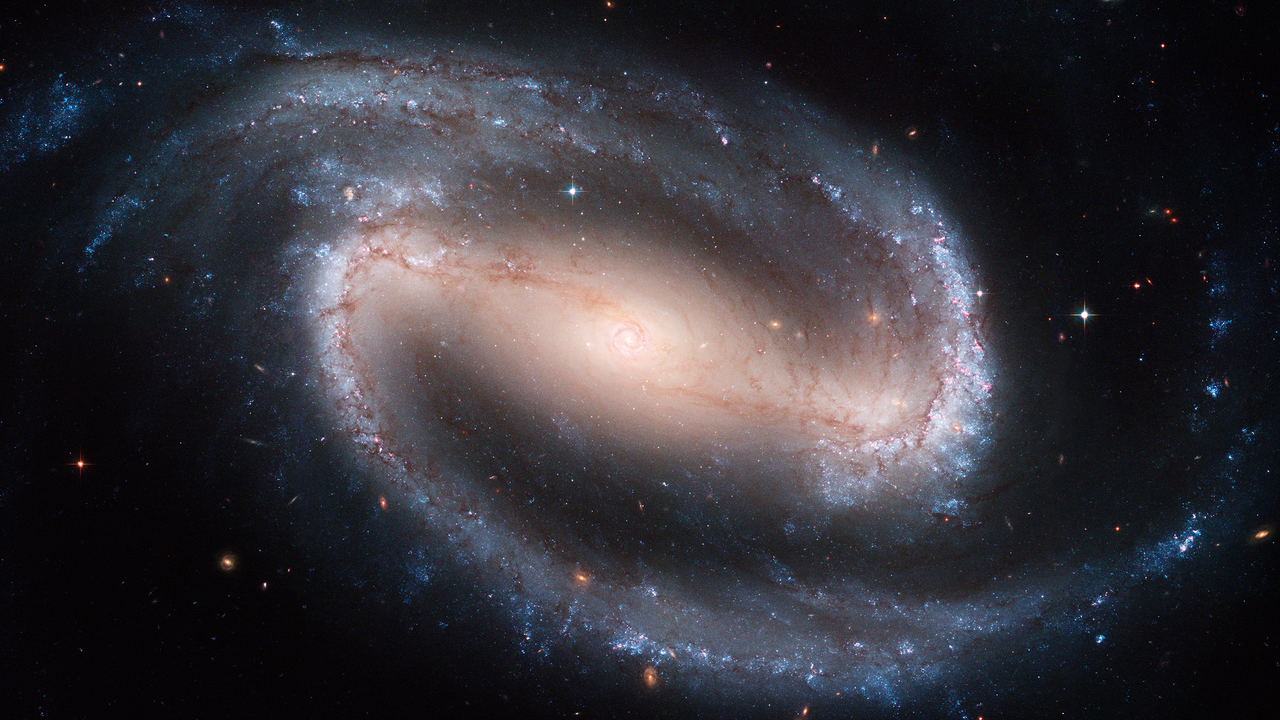
\includegraphics[width=\textwidth]{figures/NGC1300.png}
	\caption[An image of NGC 1300.]{One of the largest \glsfmtshort{hst} images ever made of a complete galaxy; an image of NGC 1300.}
	\label{fig:NGC1300}
    \imref{Credit: NASA, ESA, and The Hubble Heritage Team (STScI/AURA); \\
    Acknowledgment: P. Knezek (WIYN)}
\end{figure}
\lipsum[9-16]

Here are some more predefined acronyms to show different pages listed in the nomenclature: \gls{com}, \gls{hr}, \gls{lsst}, \gls{hst}, \gls{alma}, \gls{ska}, \gls{2mass} and \gls{cmb}.
